\documentclass[../main.tex]{subfiles}
\begin{document}
\section{Introduction}
\label{sec:introduction}
\begin{figure}
    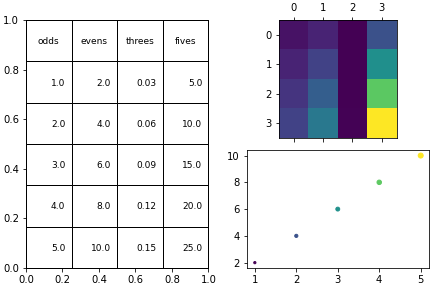
\includegraphics[width=.5\textwidth]{figures/intro/viz_same.png}
    \caption[]{Implicit in visualization is the assumption that these three representations of data are equivalent, specifically that the measurements within a variable and relations of the measurements of each variable are preserved. }
    \label{fig:viz_same}
    %% change up image to dubois or bertin or 
    
\end{figure}

\subsection{Thesis statement}
We define a visualization as a transform from data to graphic that preserves the topology of the data and faithfully map the properties of the measurement type. In fig~\ref{fig:viz_same}, we implicitly assume that the translation from table to heatmap has preserved the order of observations (the rows) and that the perceptually uniform sequential colormap has been applied such that the ordering relation on floats matches the ordering on the colormap (darker colors map to larger numbers). We also make this assumption about color in the scatter map, and that the translation to size and position on screen also respect the ordering on floats. In this work, we propose to mathematically describe the transform of data to visual space such that we can make explicit the implicit topology and types visualizations preserve. We then propose a new architecture for the Python visualization library Matplotlib \cite{hunterMatplotlib2DGraphics2007} based on these descriptions because the Matplolib artist layer is analogous to the transforms. 


\subsection{ What are the the basic requirements of a visualization library?}
Acquired codes of meaning, dubois

\section{Not all data are tables}

Tables, images (Lev), graphs (network X)

set up: dubois

theorists:
bertin, munzner, mackinlay

talk about:
matplotlib arch paper, excel/matlab arch, 
vtk \& ggplot (compare/contrast, we're blending these things) 


\subsection{Terminology}
\textcolor{blue}{Is currently C\&P'ed from my second exam so needs some messaging, but }
\begin{figure}[h!]
%%remake properly at some point
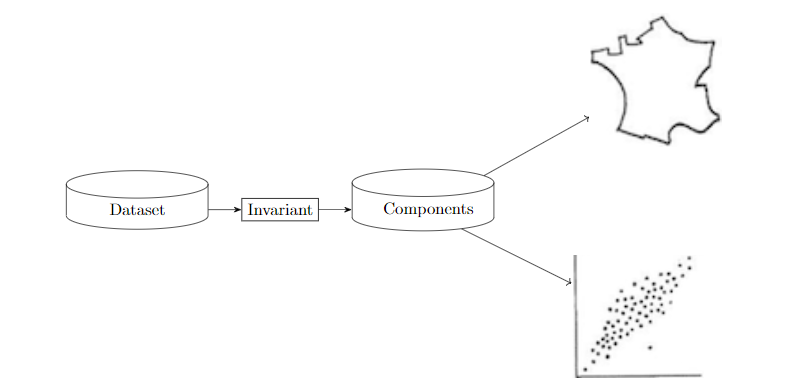
\includegraphics[width=\textwidth]{figures/intro/flowchart.png} 
\caption{To go from a dataset to a visualization, the data is subset based on a set of constraints (the invariant). The resulting subset becomes the components that are visualized, but the choice of visualization is dependent on the type and structure of the component variables.}
\label{fig:flowchart}
\end{figure}

Given a dataset, we need to decide what subset of the data to visualize. Bertin describes the set of constraints used to subset the data as the \textit{invariant}. Formally, the \textit{invariant} is the set of shared characteristics of the data being visualized. When these constraints are applied to the dataset, the resulting subset is what will become the \textit{components} of the visualization \cite{bertinSemiologyGraphicsDiagrams2011a}. 
%%rework this statement for french labor data
%%In figure~\ref{fig:iris_scatter}, the \textit{invariant} common to all the data being visualized is "sepal length", "petal length", and "species" and the \textit{components} are the measurements of these variables. 
As shown in figure~\ref{fig:flowchart}, the final step in creating a visualization is choosing how to encode the
components using retinal (visual) variables.
 

\subsubsection{Retinal (Visual) Variables}
\begin{figure}[h!]
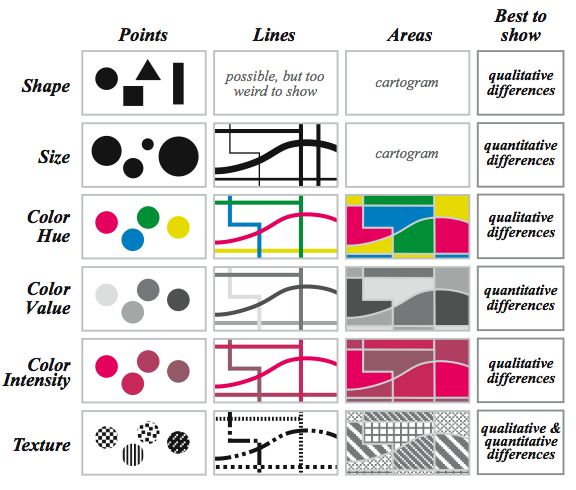
\includegraphics[width=1\textwidth]{figures/intro/retinal_variables.png}
\caption{Retinal variables are a codification of how position, size, shape, color and texture are used to illustrate variations in the \textit{components} of a visualization. This tabular form of Bertin's retinal variables is from Understanding Graphics \cite{malamedInformationDisplayTips2010} who reproduced it from \textit{Making Maps: A Visual Guide to Map Design for GIS} 
\cite{krygierMakingMapsVisual2005}}
\label{fig:retinal_variables}
\end{figure}

Figure~\ref{fig:retinal_variables} illustrates common guidelines for encoding \textit{components}, derived from what Bertin terms a retinal variable and most other visualization theorists call visual variables \cite{bertin_semiology_2011,krygier_making_2005,chambers_graphical_1983,wilkinson_grammar_2005,munzner_visualization_2014}. The columns of figure~\ref{fig:retinal_variables} correspond to the type of observation: discrete points, continuous events (e.g. a timeseries), two dimensional continuous events (e.g. a vector map). The rows of figure~\ref{fig:retinal_variables} describe ways to visualize variations in the \textit{components}; generally, quantitative components are represented by retinal variables that change quantitatively and categorical components are represented by retinal variables that vary qualitatively. In figure~\ref{fig:iris_scatter}, the hue of the marker is used to encode differentiation in species and the position of the marker is used to show variation in petal length and sepal length. The retinal variables suggest that any single visualization is limited to encoding at most about 8 or 9 components. Retinal variables provide guidelines for encoding \textit{components}, but the choice of graph is based on the type and structure of the data. 

\subsubsection{Data Type and Structure}
\label{sec:intro_data_structure}
\begin{figure}[h!]
 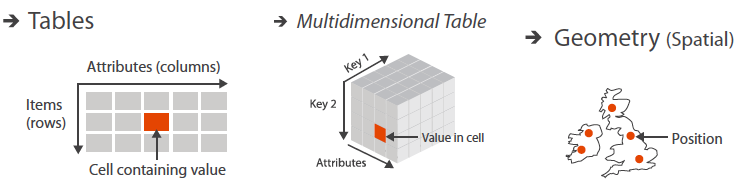
\includegraphics[width=\textwidth]{figures/intro/munzner_datatypes}
\caption{Keys are unique lookup values used to find individual observations in the dataset. Keys are positional references, and can be coordinates on a map or unique values such as a primary key in a database or a (time, latitude, longitude) index in a data cube. Image modified from a diagram from Munzner's \textit{Visualization Analysis and Design} \cite{munznerVisualizationAnalysisDesign2014}}
\label{fig:munzner_datatypes}
\end{figure}

As shown in figure~\ref{fig:flowchart}, there are multiple ways to translate data into pictures. A map is always an option, except when the observations do not have associated coordinates in a physical plane. Tamara Munzner provides a way to distinguish between these datasets using $\{key, value\}$ designations \cite{munznerVisualizationAnalysisDesign2014}. Munzner defines \textit{values} as measurements of interest in the dataset, analogous to dependent variables in statistics. She defines \textit{keys} as indexes that can be used to look up values, analogous to independent variables in statistics and dimensions in computer science. Figure~\ref{fig:munzner_datatypes} illustrates how these keys are used to look up variables in a dataset: 
\begin{itemize}
	\item map: keys are the coordinates of the points
	\item table: row index, database primary key
	\item data cube: row, column, etc. (.e.g. $i,j,k$) index
\end{itemize}

Expanding on Munzner's key and value semantics, in many datasets the keys are discrete variables like time or geophysical locations sampled from a continuous curve, surface, or field. While these observations are discrete samples from the continuous space, often the continuous (functional) characteristic\cite{ramsayFunctionalDataAnalysis2006a,mullerFunctionalVarianceProcesses2006a} of the observational space is also of interest. Besides quantitative discrete, quantitative continuous, or categorical measurement type considerations, the choice of visualization is also influenced by the measurement being on an interval, ratio, nominal, or categorical scale. 


\end{document}